% Slide mockup (16:9): metadata load that serving induces on the master.
% Input: Mooncake FAST'25 tool&agent trace (23,608 requests in 1 h, 8,596 prompt
% tokens on average, 59% cached; replayed on 16 x 8-GPU nodes). Capacity: E1.
% Build: lualatex slide_load_estimate.tex
\documentclass{article}
\usepackage{fontspec}
\setsansfont{Helvetica}
\renewcommand{\familydefault}{\sfdefault}
\usepackage{tikz}
\usetikzlibrary{arrows.meta}
\pagestyle{empty}
\definecolor{subtext}{gray}{0.35}
\begin{document}
\setbox0=\hbox{%
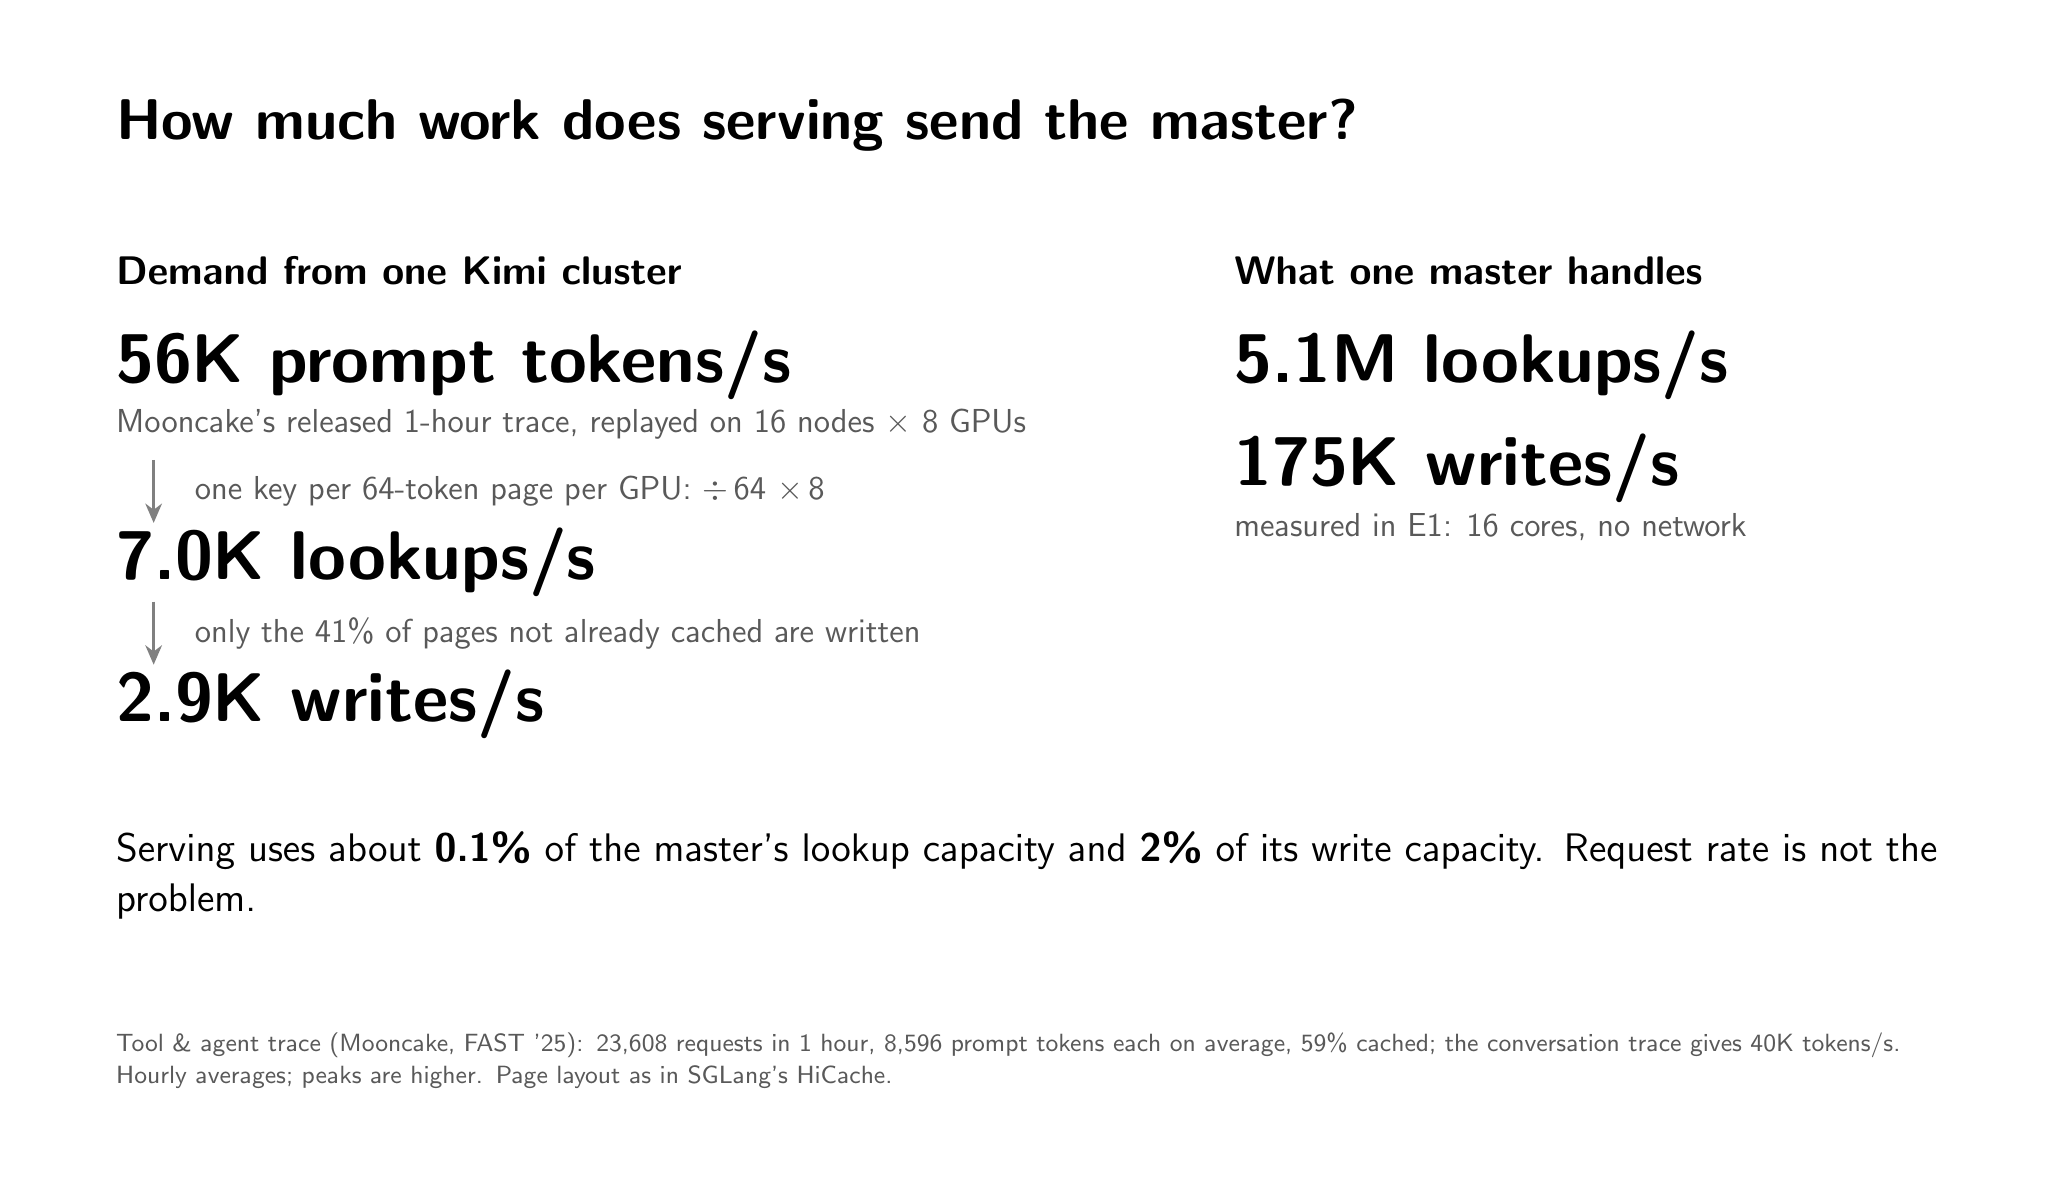
\begin{tikzpicture}[x=1cm,y=1cm]
  \path[use as bounding box] (0,0) rectangle (25.4,14.29);
  \fill[white] (0,0) rectangle (25.4,14.29);
  \tikzset{
    big/.style={anchor=west, font=\fontsize{24}{28}\selectfont\bfseries},
    why/.style={anchor=west, font=\fontsize{12.5}{15}\selectfont, text=subtext},
    hdr/.style={anchor=west, font=\fontsize{14}{17}\selectfont\bfseries},
    down/.style={-{Stealth[length=7pt,width=6pt]}, line width=1pt, draw=black!50},
  }

  \node[anchor=north west, font=\fontsize{21}{25}\selectfont\bfseries] at (1.0,13.5)
    {How much work does serving send the master?};

  % --- Demand: one Kimi cluster -------------------------------------------------
  \node[hdr] at (1.0,11.2) {Demand from one Kimi cluster};
  \node[big] at (1.0,10.0) {56K prompt tokens/s};
  \node[why] at (1.0,9.25) {Mooncake's released 1-hour trace, replayed on 16 nodes $\times$ 8 GPUs};
  \draw[down] (1.6,8.8) -- (1.6,8.0);
  \node[why] at (2.0,8.4) {one key per 64-token page per GPU: $\div$\,64 $\times$\,8};
  \node[big] at (1.0,7.5) {7.0K lookups/s};
  \draw[down] (1.6,7.0) -- (1.6,6.2);
  \node[why] at (2.0,6.6) {only the 41\% of pages not already cached are written};
  \node[big] at (1.0,5.7) {2.9K writes/s};

  % --- Capacity: one master --------------------------------------------------------
  \node[hdr] at (15.2,11.2) {What one master handles};
  \node[big] at (15.2,10.0) {5.1M lookups/s};
  \node[big] at (15.2,8.7) {175K writes/s};
  \node[why] at (15.2,7.95) {measured in E1: 16 cores, no network};

  % --- Result ---------------------------------------------------------------------
  \node[anchor=north west, text width=23.4cm, font=\fontsize{14}{18}\selectfont] at (1.0,4.2)
    {Serving uses about \textbf{0.1\%} of the master's lookup capacity and \textbf{2\%} of its write capacity.
     Request rate is not the problem.};

  \node[anchor=south west, text width=23.4cm, font=\fontsize{9.5}{11.5}\selectfont, text=subtext] at (1.0,0.7)
    {Tool \& agent trace (Mooncake, FAST '25): 23,608 requests in 1 hour, 8,596 prompt tokens each on average, 59\% cached;
     the conversation trace gives 40K tokens/s. Hourly averages; peaks are higher. Page layout as in SGLang's HiCache.};
\end{tikzpicture}}%
\pdfvariable horigin=0pt
\pdfvariable vorigin=0pt
\pagewidth=\wd0
\pageheight=\dimexpr\ht0+\dp0\relax
\shipout\box0
\end{document}
